\section{Auction-SC Framework}
\label{sec:onlinealgo}

In practice, an SC system works similar to a \emph{complex event processing (CEP)} engine \cite{Luckham01} where new tasks arrive at the SC-Server as an input stream. With a real-world SC scenario, the SC-Server will find out about a task and its properties only when it is released. The complexity of the many-to-many matching in addition to the need for immediacy (e.g., Uber) render the batch scheme impractical for real-world scenarios. Furthermore, in an online centralized SC-Server scheduling multiple workers becomes the bottleneck and hence, real-time assignment is not guaranteed.

In this section we introduce Auction-SC which has neither shortcomings and generates real-time online assignments by splitting the matching and scheduling responsibilities between the server and the workers, respectively. This allows Auction-SC to scale up orders of magnitude higher than a centralized SC-Server (see \cref{subsec:exp_scale}. First we explain the auction framework and how tasks are dispatched to workers. Next, we discuss how workers compute their bids and at the end we provide a cost analysis of this framework.

\subsection{Task Dispatchment in Auction-SC}

%\subsection{Batched vs. Online Assignment}
%In practice, an SC system works similar to a \emph{complex event processing (CEP)} engine \cite{Luckham01} where new tasks arrive at the SC-Server as an input \textit{stream}. In a real-world SC scenario, the SC-Server will find out about a task and its properties only when its released. At this time the SC-Server should either immediately assign the task to the worker (online assignment) or wait for more tasks to arrive and assign all the recently released tasks at once (batched assignment). 

%As explained earlier, at each point in time, an SC worker has a schedule. Finding a schedule that satisfies both spatial and temporal constraints of the tasks assigned to every worker, is computationally expensive when we have a large number of workers. To overcome the complexity of the problem at scale, almost every prior work on task assignment in SC uses the batched assignment schema. While the server is busy doing the assignment and scheduling for the current batch of tasks, the next batch of tasks arrive at the server. Once the server completes processing the previous batch it start processing the tasks that have been queued. It is worth mentioning that in batched assignment, matching the tasks to the workers itself is a many-to-many matching where there are multiple workers and multiple tasks.

%On the other hand, in the online assignment schema a task is assigned to a worker as soon as it arrives at the SC-Server. The SC-Server should be able to do the matching and scheduling in real-time to be able to process the next incoming task in time. At each point of time the SC-Server is processing only one task. Hence, the matching phase become a one-to-many matching where there are multiple workers and only one task. Consequently, the complex many-to-many matching phase in batched assignment is reduced to only selecting the best worker, in the online assignment schema.

%We end this subsection with a comparison between the two schemas. One advantage of batched assignment is that it is processing multiple tasks at a time. This means the SC-Server can possibly make a better assignment when knowing about all the tasks in a batch compared to when it processes the same set of tasks one at a time, knowing only about the single task that is being processed at each point of time. However, in batched assignment, this excess of information comes at the cost of every task losing a portion of the time it is available before its deadline. For example, task \textit{a} arrives at the server at time \textit{t} with a deadline at \textit{t+30min}. We assume that the SC-Server finishes processing the previous batch at time \textit{t+15min}. In this example, by the time the SC-Server starts processing the batch that contains \textit{a}, half of the time between \textit{a}'s release and its deadline has already past. Intuitively, this means the chances of \textit{a} being assigned to a worker is cut in half. In addition, we already explained that the matching phase is more complex in batched assignment compared to online assignment. More importantly, if for some reason scalability is not an issue, in many real-world SC environments, the requester requires a real-time response w.r.t. whether the requested task has been assigned to a worker or not. For example, we can consider ride sharing applications like Uber and Lyft as SC systems where the tasks are the ride requests and the workers are the drivers. In such systems, as soon as a rider requests a ride, they want to know if any available driver is going to be able to service them. A batched assignment schema will simply not work in such systems since the requester cannot wait for a long amount of time until the server processes its request.

%\subsection{Auction-SC Algorithms}
%In online assignment the matching phase is reduced to only selecting the best worker among \textit{eligible} workers which is defined as:

%In a centralized implementation, when a new task arrives, the SC-Server has to perform the scheduling phase for all eligible workers. This means that it has to compute a potential best schedule for those workers considering that the new task is assigned to them. When presented with a large number of workers this can become computationally expensive. In this paper we propose an auction-based framework, Auction-SC, that overcomes the high computation cost of scheduling by distributing the process among workers. In the remainder of this section we discuss the details of Auction-SC and analyze the computation and communication costs of it compared to a centralized approach.

Auction methods have been effectively used for assignment problems in dynamic multi-agent environments \cite{Mehta05,Lagoudakis04}. The main advantage of auction methods are their simplicity and the fact that they allow for a decentralized implementation. Auction-SC considers workers as bidders and tasks as goods. Furthermore, the SC-Server plays the role of a central auctioneer in Auction-SC. At a very high level, in Auction-SC, once a new tasks is submitted to the SC-Server (auctioneer), the server presents the task to the workers (bidders). Depending on the \textit{bidding rule}, which is common among all workers, each worker computes its own bid and submits the bid to the server. The bidding process is performed as a \textit{sealed-bid auction} where workers simultaneously submit bids and no other workers knows how much the other workers have bid. The SC-Server selects the worker with either the lowest or highest bid (depending on the bidding rule) as the winner and matches the task with the worker.

Broadcasting every incoming task to all available workers incurs a large communication cost on the system. Auction-SC lowers the communication cost by only sending any incoming task to \textit{eligible workers} that are define as:

\begin{definition} [Eligible Worker]
An available worker w is said to be eligible for performing a newly released task t, if and only if:
\begin{equation*}
distance(w, t) \leq w.d - t.r \wedge distance(w, t) \leq t.d - t.r
\end{equation*}
\end{definition}

\noindent In other words, an available worker \textit{w} is eligible for performing task \textit{t}, if it has enough time to reach the location of \textit{t} before either \textit{t} expires or \textit{w} leaves the system. The SC-Server maintains a spatial index on the location of the workers. With Auction-SC, we use a grid index since (1) the workers have to send updated locations to the server only if they change cells and (2) the server does not need to know the exact location of the worker to be able to filter out non-eligible workers. A detailed analysis of the communication cost is presented at the end of this section.

\begin{algorithm}
\caption{OnlineTASC($W, t$)}
\label{algo:OnlineTASC}
\begin{algorithmic}[1]
\REQUIRE $W$ is the set of currently available workers and $t$ is a task the has just released
\ENSURE Either $w \in W$ as the worker task $t$ should be assigned to or \emph{null} if no worker is selected
\STATE $w_{selected} = $ \emph{null}
\STATE $Bids = \emptyset$
\FOR{$w \in W_t$} \label{line:loop_start}
	\STATE $bid = w$.ComputeBid$(t)$ \label{line:compute}
	\STATE $Bids \leftarrow \left\langle w, bid \right\rangle$
\ENDFOR \label{line:loop_end}
\STATE $w_{selected} = $ SelectBestBid$(Bids)$ \label{line:select}
\RETURN $w_{selected}$
\end{algorithmic}
\end{algorithm}

\cref{algo:OnlineTASC} outlines the process of assigning an incoming task $t$. $W_t$ in line \ref{line:loop_start} is the set of eligible workers for task \textit{t}. Notice that all the iterations of the \textbf{for} loop in \cref{algo:OnlineTASC} (lines \ref{line:loop_start}-\ref{line:loop_end}) run in parallel. The \emph{ComputeBid()} method (line \ref{line:compute}) that each worker executes depends on the implemented bidding rule. Similarly, the \emph{SelectBestBid()} method (line \ref{line:select}) returns the worker with either the highest or lowest bid. In case of a tie, the \emph{SelectBestBid()} method, randomly selects one worker among the ones with optimal bid.

\subsection{Worker's Bid Computation}

With Auction-SC, every worker computes its bid using a predefined bidding rule. A worker's bid represents how good it is to be matched with the task. When computing a bid for a task, the workers have no knowledge about other tasks that might arrive in the future. Consequently, they have to make a greedy decision based on their current status. First we introduce four simple bidding rules based on heuristics that are used for other problems that seem to be similar to task assignment in SC, hence we call them non-SC rules. These problems do not consider either the spatial or temporal dynamism of SC. We use non-SC rules in the experiments to show the importance of both spatial and temporal aspects of SC. The four non-SC rules used in our experiments are:

\noindent\textbf{Random (Rnd)}:
As a baseline approach, we consider a rule where every eligible worker submits a bid of value 1. The SC-Server selects the winner randomly from the set of eligible workers.

\noindent\textbf{Ranking (Rnk)}:
Based on the ideas in \emph{Online Bipartite Matching} \cite{Karp90}, the workers are ranked from 1 to $n$ (the workers' order do not change over time). Each eligible worker submits a bid of value 1 and the SC-Server selects the eligible worker with the lowest rank as the winner. This heuristic does not consider either spatial or temporal aspects of SC.

\noindent\textbf{Nearest Neighbor (NN)}:
Similar to the the \emph{Spatial Matching} problem \cite{Wong07}, for this bidding rule we give priority to the closest worker to the location of the task. This means a worker closer to the location of the incoming task is better sutied to perform the task compared to a worker farther away. To compute a bid, each worker needs to compute the distance between the location of the task and its own location and submit the computed distance as its bid. Once every worker has submitted its bid, the SC-Server chooses the worker with the minimum bid as the winner. This bidding rule only considers spatial constraints of SC.

\noindent\textbf{Most Free Time (MFT)}:
In this bidding rule, based on the ideas in \emph{Online Scheduling} \cite{Lee13}, we give priority to workers that have more time before they leave the system. At each point of time, a worker computes its \emph{free time} as the duration between the time it finishes its current schedule and the time it leaves the system. Each worker submits a bid equal to its \emph{free time} and the SC-Server selects the worker with the highest bid as the winner. This bidding rule only considers the temporal dynamism of SC.
 
In addition to the four non-SC rules, we propose two bidding rules that consider both spatial and temporal constraints of SC and hence, we call them SC rules. The intuition behind the first bidding rule is that the less time a worker spends completing an incoming task, the higher the chances are that it is available in the future to perform more tasks. Our second SC rule, tends to move workers to areas that there is a higher chance for a task to show up in the future. We describe how workers compute their bids and how the server selects the winner in the following.\\

\noindent \textbf{Best Insertion (BI)}: 
Intuitively, if a worker spends less time to complete a task it will likely have more time for performing other tasks. In BI, the server gives priority to workers that can better insert the incoming task into their schedules. Auction-SC considers the \textit{extra time} each worker will need to complete the new task in addition to its current schedule.

Each worker starts with finding a potential optimal schedule where the new task is added to its current schedule. For this process, the worker uses a branch and bound algorithm to check all possible orders of its uncompleted tasks in addition to the new task. Running an exhaustive search for large number of tasks can be time consuming. However, in our experiments on both real world and synthetic data, we realized that the number of uncompleted tasks at each point of time for each worker, remains in a range where even the exhaustive search can be done in real-time for a single worker. The reason is that, as time passes and new tasks arrive, the worker also completes other tasks and removes them from its schedule. In cases where computing the bid takes too long, we can replace this computation with an approximate algorithm (e.g., the Nearest Insertion algorithm \cite{Rosenkrantz74}). In our experiments, we show that running an approximate algorithm for the scheduling phase, reduces the accuracy of the assignment by less than 5\%.

In order to compute a bid, each worker computes the finish time of the potential optimal schedule in case it is matched with the new task ($f_2$). The worker also knows the finish time of its current schedule $(f_1)$. For each worker, $f_2-f_1$ is the \textit{extra time} it requires to complete the new task in addition to tasks in its current schedule. Therefore the bid each worker submits to the SC-Server is equal to $f_2 - f_1$. After receiving the bids from every worker, the SC-Server assigns the task to the worker with the lowest bid.\\

\noindent \textbf{Best Distribution (BD)}: 
BI does not consider the spatial distribution of tasks. It might be beneficial to assign a task located at a task-dense area to a worker with high remaining availability, even if the worker has to move from its current location significantly. The general idea behind this rule is to try to move workers to locations that have a higher chance of having a task in the future. Ideally, we want the spatial distribution of the \textit{available} workers $(S_W)$ to be as close as possible to the \textit{overall} spatial distribution of the tasks $(S_T)$.

One can argue that knowing $S_T$ contradicts the assumption that the SC-Server has no spatiotemporal knowledge about future tasks. Even if the SC-Server knows $S_T$, it does not mean it also knows the exact locations at which the tasks are going to be released. Nevertheless, with Auction-SC we do not make the assumption that $S_T$ is known a priori. Instead, we assume the SC-Server starts with an empty distribution and keeps updating it as new tasks arrive.

For $S_W$ and $S_T$ we use a grid index similar to the one Auction-SC maintains for choosing eligible workers when a task arrives. For each event occurring inside a cell, we add to the weight of that cell. To compute $S_T$, for every task we add a value of 1 to the cell containing the task. As for $S_W$, we need to consider the \textit{availability} of the worker. For example, if the maximum number of tasks worker $w$ can perform is $n$, and it already has been assigned $m$ tasks, we say the availability of worker $w$ is $n-m$. In this case, when computing $S_W$, we add $n-m$ units to the cell covering $w$. For both $S_T$ and $S_W$, by normalizing the weights of the cells, we can compute the probability of an event occurring in each cell. In addition to the probability of each cell, the gird index keeps track of the center point of each cell in order to find the distance between two cells.

Having $S_W$ and $S_T$, we need a metric to determine the closeness of these two distributions. Several methods have been used to compute the similarity between two distributions. Among the more commonly used methods, we can name the Kullback-Leibler divergence \cite{Kullback51} and Jensen-Shannon divergence \cite{Lin91}. The problem with these methods is that they do not take the distance between the cells into consideration. For example, \cref{fig:sdist} shows two spatial distribution for two tasks (red dots) and two workers (blue squares). Clearly, the distribution of workers in \cref{fig:sdist2} is more similar to $S_T$ compared to \cref{fig:sdist1}. However, with the Jensen-Shannon divergence metric, $JSD(S_T, S_{W_1})$ is equal to $JSD(S_T, S_{W_2})$. Considering the Kullback-Leibler divergence or any other metric that does not take into account the spatial relationship between the cells, ends up with the same results.

\begin{figure}[t]
    \centering
    \subfigure[Distribution 1]{
        \label{fig:sdist1}
        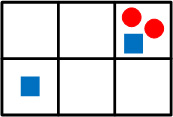
\includegraphics[scale=0.35]{figures/sDist1.jpg} }
    \subfigure[Distribution 2]{
        \label{fig:sdist2}
        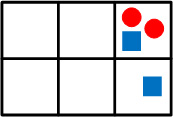
\includegraphics[scale=0.35]{figures/sDist2.jpg}
    }
    \vspace{-0.1in}
    \caption{Two spatial distributions for tasks and workers}
    \label{fig:sdist}
\end{figure}

In this paper, we use the \textit{Earth Mover's Distance} metric since it has the ability to incorporate the spatial aspect of the distributions when computing their similarity.

\begin{definition}[Earth Mover's Distance]
The Earth Mover's Distance (EMD) is a measure of distance between two probability distributions over a region $D$. If the distributions are interpreted as two different ways of piling up a certain amount of dirt over region $D$, the EMD is the minimum cost of turning one pile into the other; where the cost is assumed to be the amount of dirt moved, times the distance by which it is moved \cite{Rubner98}.
\end{definition}

If we want to compute the EMD between two distributions $A$ and $B$, for each grid cell $i$, we call cell $i$ a supplier iff $P_A(i) > P_B(i)$ and a consumer iff $P_A(i) < P_B(i)$. If $P_A(i) = P_B(i)$, cell $i$ is neither a supplier nor a consumer. For each supplier $i$, we say $a_i = P_A(i) - P_B(i)$ is the total supply of $i$. Also, the total demand for consumer $j$ is shown as $b_j = P_B(j) - P_A(j)$. Now we can model the problem as a bipartite network flow problem where on one side we have the supplier nodes and on the other side we have consumer nodes. The weight of each edge $c_{ij}$ between supplier $i$ and consumer $j$, is the cost of moving one unit of mass from $i$ to $j$.  Consequently, finding EMD reduces to finding the \textit{Minimum Cost Flow} for this bipartite graph. The Minimum Cost Flow problem can be formalized as the following linear programming problem:

%\begin{figure}[t]
%  \centering
%  \label{fig:MinFlow}
%  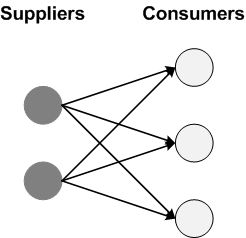
\includegraphics[scale=0.25]{figures/MinFlow.png}
%  \caption{Example of MinFlow Problem}
%\end{figure}

\setcounter{equation}{0}
\begin{alignat}{2}
\mathbf{minimize}&\mathrlap{\sum_{i \in \mathcal{I}} \sum_{j \in \mathcal{J}} c_{ij}.f_{ij}} \notag\\
\mathbf{subject\ to:}&\phantom{{a}={a}} f_{ij} && \geq 0 \ \quad\quad i \in \mathcal{I}, j \in \mathcal{J}\\
&\phantom{{a}}\sum_{i \in \mathcal{I}} f_{ij} &&= b_j \quad\quad j \in \mathcal{J}\\
&\phantom{{a}}\sum_{j \in \mathcal{J}} f_{ij} &&\leq a_i \quad\quad i \in \mathcal{I}
\end{alignat}

%More generally, for any graph $G = (V, E)$ we can assign an integer $b(i)$ to each node in the graph, which indicates the supply (or demand) of the node if $b(i) > 0$ (or $b(i) < 0$) . Then we can rewrite the linear programming problem as: 

%\setcounter{equation}{0}
%\begin{alignat}{2}
%\mathbf{minimize}&\mathrlap{\sum_{(i,j) \in \mathcal{E}} c_{ij}.f_{ij}} \notag\\
%\mathbf{subject\ to:}&\phantom{{a}={a}{a}={a}{a}={a}{a}} f_{ij} && \geq 0 \ \quad\quad (i,j) \in \mathcal{E}\\
%&\sum_{j:(j,i) \in \mathcal{E}} f_{ij} - \sum_{j:(i,j) \in \mathcal{E}} f_{ij} &&= b(i) \quad\quad i \in \mathcal{V}
%\end{alignat}

\noindent We can solve this LP problem efficiently using the simplex method \cite{Dantzig90}.

We assume the SC-Server maintains $S_W$ and $S_T$ and shares it with the eligible workers. First, each worker has to compute a potential schedule by inserting the incoming task to its current schedule. If the worker is able to find a new schedule, it can locally modify $S_W$ considering how its location and availability changes in the potential schedule, i.e., $S_{W}'$. Subsequently, the worker computes the EMD between $S_{W}'$ and $S_T$ and submits the value as its own bid. The SC-Server selects the worker with the lowest bid as the winner.

\begin{algorithm}[h]
\caption{EMDCost($P, Q$)}
\label{algo:emd}
\begin{algorithmic}[1]
\REQUIRE \emph{P} and \emph{Q} as two grid distributions
\ENSURE \emph{cost} is EMD cost between distributions \emph{P} and \emph{Q}
\STATE $suppliers = \emptyset$
\STATE $consumers = \emptyset$
\FOR{$cell = 0$ to $P.size$}\label{ln:for1_s}
	\STATE $diff = P(cell).prob - Q(cell).prob$
	\IF{$ diff > 0$}
		\STATE $suppliers \leftarrow$ new Node($diff, P(cell).center$)
	\ELSE
		\STATE $consumers \leftarrow$ new Node($diff, P(cell).center$)
	\ENDIF
\ENDFOR\label{ln:for1_e}
\STATE $edges = \emptyset$
\FOR{$s$ in $suppliers$}\label{ln:for2_s}
	\FOR{$c$ in $consumers$}
		\STATE $d =$ dist($s.center, c.center$)
		\STATE $edges \leftarrow$ new Edge($s, c, d$)
	\ENDFOR
\ENDFOR\label{ln:for2_e}
\STATE $emdGraph =$ new Graph($suppliers, consumers, edges$)
\STATE $flowGraph = emdGraph$.FindMinFlow()\label{ln:min_flow}
\STATE $cost = 0$
\FOR{$e$ in $flowGraph.edges$}
	\STATE $cost += (e.flow \times e.cost)$
\ENDFOR
\RETURN $cost$
\end{algorithmic}
\end{algorithm}

\cref{algo:emd} outlines the process of finding the EMD cost between two distributions $P$ and $Q$. First we divide the cells our spatial distributions into a \textit{supplier} set and a \textit{consumer set} (Lines~\ref{ln:for1_s}-\ref{ln:for1_e}). Then we connect each supplier node to every consumer node such that the distance between the two nodes is equal to the distance of their corresponding cells (Line~\ref{ln:for2_s}-\ref{ln:for2_e}). The \textit{FindMinFlow()} method in Line~\ref{ln:min_flow} executes the linear programming problem discussed earlier.

\subsection{Cost Analysis}

We end the discussion on Auction-SC with a detailed analysis of the communication cost in this framework. Communication cost can be looked at from two different perspectives; response time and throughput. With Auction-SC, once the task arrives at the SC-Server, it is \textit{broadcast} to a number of workers. Therefore, the SC-Server can send all messages (/packets) in parallel at the same time. In return, all workers are submitting their bids in parallel as well. Considering current network transmission speeds, even in cellular networks, the response time of transmitting a single packet of data in Auction-SC is negligible.

The other aspect of communication cost analysis is the throughput of the network. Specially when at scale, the increase in the number of sent messages can saturate the network bandwidth and cause trouble. In a centralized architecture, tasks are not broadcast to workers and there is no bid submission. Hence it seems that communication cost is not a factor in a centralized approach. However, due to the dynamism of SC, coordination between the workers and the centralized server is inevitable and they need to communicate with each other. Here we show that with regard to the number of messages transmitted between the workers and the SC-Server, there is not much difference between a centralized approach and Auction-SC.

As explained earlier, with Auction-SC we implement a grid index that keeps track of the location of available workers. The SC-Server uses this grid index to identify eligible workers and only broadcast the new task to them. The worker has to notify the server about its location only if its movement causes it to switch cells. We assume, on average a workers switches cells $\bar{\alpha}$ times and show the total number of workers with $n$. Subsequently, the number of messages transmitted to notify the SC-Server about a cell change is $\bar{\alpha}.n$. Upon the arrival of a new task \textit{t}, the SC-Server identifies all the cells within \textit{t.d} distance of \textit{t}'s location and broadcasts the task to workers only in those cells. Assuming on average there are $\bar{n_e}$ eligible workers for each task, we can compute the number of transmitted messages as:
\begin{equation*}
\left| M_{Auction} \right| = \bar{\alpha}.n + 2|T|\bar{n_e}
\end{equation*}

On the other hand, In a centralized approach, the SC-Server does all the computation and assigns the new task to the best workers by itself. In order to compute a potential new schedule for each worker, the server has to know the \textit{exact} location of every worker. One idea is for the SC-Server to internally keep a spatial index on the exact location of the workers and use it to retrieve the exact location of workers when necessary. The problem with such a spatial index is that even if only 10\% of the workers move and update their locations frequently, it can take up to 20 seconds to update the spatial index \cite{Akdogan14} which is not acceptable in a real-time system. The other option is for the SC-Server to query the exact location of the eligible workers when it wants to compute their potential schedule. To prevent querying all available workers, we assume the centralized server utilizes a grid index as well. Therefore, it can only query the eligible workers for their exact location once a task arrives. Consequently, upon arrival of each task and for each eligible worker, one message is sent from the server to ask for the exact location and one message is sent back to the server with the exact location. Similarly, we can compute the total number of transmitted messages as:
\begin{equation*}
\left| M_{Centralized} \right| = \bar{\alpha}.n + 2|T|\bar{n_e}
\end{equation*}
\noindent Similar to Auction-SC, $\bar{\alpha}.n$ is the total number of messages sent to the server to change the workers' cells. We can see the number of messages transmitted in a centralized server is similar to those with Auction-SC. Thus, when compared to a centralized architecture, Auction-SC does not increase the throughput of the network. It should be mentioned that in the BD approach, since $S_W$ and $S_T$ should be broadcast to eligible workers, it incurs a slightly higher communication cost and as it can be seen in the experiments, BD becomes less scalable than BI.